%% bare_conf.tex
%% V1.4b
%% 2015/08/26
%% by Michael Shell
%% See:
%% http://www.michaelshell.org/
%% for current contact information.
%%
%% This is a skeleton file demonstrating the use of IEEEtran.cls
%% (requires IEEEtran.cls version 1.8b or later) with an IEEE
%% conference paper.
%%
%% Support sites:
%% http://www.michaelshell.org/tex/ieeetran/
%% http://www.ctan.org/pkg/ieeetran
%% and
%% http://www.ieee.org/

%%*************************************************************************
%% Legal Notice:
%% This code is offered as-is without any warranty either expressed or
%% implied; without even the implied warranty of MERCHANTABILITY or
%% FITNESS FOR A PARTICULAR PURPOSE!
%% User assumes all risk.
%% In no event shall the IEEE or any contributor to this code be liable for
%% any damages or losses, including, but not limited to, incidental,
%% consequential, or any other damages, resulting from the use or misuse
%% of any information contained here.
%%
%% All comments are the opinions of their respective authors and are not
%% necessarily endorsed by the IEEE.
%%
%% This work is distributed under the LaTeX Project Public License (LPPL)
%% ( http://www.latex-project.org/ ) version 1.3, and may be freely used,
%% distributed and modified. A copy of the LPPL, version 1.3, is included
%% in the base LaTeX documentation of all distributions of LaTeX released
%% 2003/12/01 or later.
%% Retain all contribution notices and credits.
%% ** Modified files should be clearly indicated as such, including  **
%% ** renaming them and changing author support contact information. **
%%*************************************************************************


% *** Authors should verify (and, if needed, correct) their LaTeX system  ***
% *** with the testflow diagnostic prior to trusting their LaTeX platform ***
% *** with production work. The IEEE's font choices and paper sizes can   ***
% *** trigger bugs that do not appear when using other class files.       ***                          ***
% The testflow support page is at:
% http://www.michaelshell.org/tex/testflow/



\documentclass[conference]{IEEEtran}
% Some Computer Society conferences also require the compsoc mode option,
% but others use the standard conference format.
%
% If IEEEtran.cls has not been installed into the LaTeX system files,
% manually specify the path to it like:
% \documentclass[conference]{../sty/IEEEtran}





% Some very useful LaTeX packages include:
% (uncomment the ones you want to load)

\usepackage[left=2cm,right=2cm,bottom=3cm,top=2.5cm]{geometry}

\let\proof\relax
\let\endproof\relax

\usepackage{amsmath}
\usepackage{amsfonts}
\usepackage{amsthm}
\usepackage{amssymb}
\usepackage{mathtools}
\usepackage{soul}
\usepackage{xspace}
\usepackage{xcolor}
\usepackage{enumitem}
\usepackage{hyperref}
\usepackage[capitalise]{cleveref}
\usepackage{booktabs}
\usepackage{tabularx}
\usepackage{mdframed}
\usepackage{multirow}
\usepackage{float}
\usepackage[linesnumbered,ruled,vlined]{algorithm2e}
\usepackage{algpseudocode}
\usepackage{subcaption}
\usepackage{multirow}
\usepackage{makecell}
\usepackage[all,cmtip]{xy}
\usepackage{graphicx}
\usepackage{framed}

% \pagespttyle{plain}


\setul{1ex}{.5pt}

\hypersetup{
    % pdftitle={},
    % pdfauthor={},
    colorlinks=true,
    linkcolor=black,
    citecolor=black,
    pdfstartview=FitH,
    pdfpagemode=UseOutlines,
    pdfpagelayout=OneColumn,
}

\setcounter{tocdepth}{2}

\mdfdefinestyle{figstyle}{ %
	linecolor=black!7, %
	backgroundcolor=black!7, %
	innertopmargin=10pt, %
	innerleftmargin=25pt, %
	innerrightmargin=25pt, %
	innerbottommargin=10pt %
}

\newtheorem{theorem}{Theorem}
\newtheorem{lemma}{Lemma}
\newtheorem{hypothesis}[theorem]{Hypothesis}
\newtheorem{corollary}[theorem]{Corollary}
\newtheorem{construction}{Construction}

\theoremstyle{definition}
\newtheorem{action}{Group Action}
\newtheorem{definition}[theorem]{Definition}
\newtheorem{assumption}{Assumption}
\newtheorem{observation}{Observation}
\newtheorem{fact}{Fact}
\newtheorem{remark}[theorem]{Remark}

\newcommand{\bra}[1]{\langle{#1}|}
\newcommand{\ket}[1]{|{#1}\rangle}
\newcommand{\ip}[2]{\langle{#1}, {#2}\rangle}
\newcommand{\braket}[2]{\langle{#1}|{#2}\rangle}
\newcommand{\mode}[1]{\textnormal{\textsf{#1}}}
\renewcommand{\vec}[1]{\mathbf{#1}}
\newcommand{\F}{\mathbb{F}}
\newcommand{\K}{\mathbb{K}}
\renewcommand{\P}{\mathbb{P}}
\newcommand{\Z}{\mathbb{Z}}
\newcommand{\R}{\mathbb{R}}
\newcommand{\N}{\mathbb{N}}
\newcommand{\Matrix}{\mathrm{M}}
\newcommand{\Tensor}{\mathrm{T}}
\newcommand{\id}{\mathrm{id}}
\newcommand{\ATF}{\mathrm{ATF}}
\newcommand{\rk}{\mathrm{rank}}
\newcommand{\probsty}[1]{\textsf{#1}\xspace}
\newcommand{\GI}{\probsty{GI}}
\newcommand{\PK}{\mathrm{PK}}
\newcommand{\SK}{\mathrm{SK}}

\newcommand{\CFI}{\probsty{CFI}}
\newcommand{\ID}{\probsty{ID}}
\newcommand{\QFMI}{\probsty{QFMI}}
\newcommand{\pGpI}{$p$\probsty{GpI}}
\newcommand{\GMW}{\probsty{GMW}}
\newcommand{\Alteq}{\probsty{ALTEQ}}
\newcommand{\DATFE}{\probsty{DATFE}}
\newcommand{\MATFE}{\probsty{MATFE}}
\newcommand{\PATFE}{\probsty{PATFE}}
\newcommand{\Exp}{\probsty{Exp}}
\newcommand{\ATFA}{\probsty{ATFA}}
\newcommand{\EUFCMA}{\probsty{EUF-CMA}}
\newcommand{\sEUFCMA}{\probsty{sEUF-CMA}}
\newcommand{\EUFNMA}{\probsty{EUFNMA}}
\newcommand{\CROATFE}{\probsty{$C$-PR-psATFE-RO}}
\newcommand{\ROATFE}{\probsty{PR-psATFE-RO}}
\newcommand{\FS}{\probsty{FS}}
\newcommand{\PI}{\probsty{PI}}
\newcommand{\TIp}{\probsty{TI}}
\newcommand{\DTI}{\probsty{DTI}}
\newcommand{\TTI}{\probsty{3TI}}
\newcommand{\gainv}{\probsty{GA-Inv}}
\newcommand{\gapr}{\probsty{GA-PR}}
\newcommand{\msg}{M}
\newcommand{\cB}{\mathcal{B}}
\newcommand{\cA}{\mathcal{A}}
\newcommand{\cI}{\mathcal{I}}
\newcommand{\cX}{\mathcal{X}}
\newcommand{\cY}{\mathcal{Y}}
\newcommand{\cZ}{\mathcal{Z}}
\newcommand{\cK}{\mathcal{K}}
\newcommand{\cP}{\mathcal{P}}
\newcommand{\cS}{\mathcal{S}}
\newcommand{\cD}{\mathcal{D}}
\newcommand{\tA}{\mathtt{A}}
\newcommand{\Tr}{\mathrm{Tr}}

\newcommand{\sampcost}{\textsf{samp-cost}}
\newcommand{\colcost}{\textsf{col-cost}}
\newcommand{\invcost}{\textsf{inv-cost}}
\newcommand{\mrkcost}{\textsf{minrank-cost}}

\newcommand{\tB}{\mathtt{B}}

%\newcommand{\M}{\mathrm{M}}
\newcommand{\diag}{\mathrm{diag}}
\newcommand{\gpmul}{\circ}
\newcommand{\gpact}{\ast}
\newcommand{\class}[1]{\ensuremath{\mathrm{#1}}\xspace}
\newcommand{\NP}{\class{NP}}
\newcommand{\TI}{\class{TI}}
\newcommand{\coNP}{\class{coNP}}
%\newcommand{\coAM}{\class{coAM}} %cryptocode

%\newcommand{\secpar}{\lambda} %cryptocode
\newcommand{\usecpar}{1^\secpar}
\newcommand{\veps}{\varepsilon}
\newcommand{\bit}{\{0,1\}}


\newcommand{\FG}{\mathrm{FG}}


\newcommand{\abbrsty}[1]{\ensuremath{\mathrm{#1}}\xspace}
\newcommand{\OWA}{\abbrsty{OWA}}
\newcommand{\PRA}{\abbrsty{PRA}}
\newcommand{\PROD}{\abbrsty{PROD}}
\newcommand{\INV}{\abbrsty{INV}}
\newcommand{\QRO}{\abbrsty{QRO}}
\newcommand{\GLAT}{\abbrsty{GLAT}}

\newcommand{\pg}{\mathcal{G}}
\newcommand{\cm}{\mathcal{CM}}
\newcommand{\qdm}{\mathcal{QDM}}
\newcommand{\params}{\texttt{params}}
\newcommand{\attack}{\mathcal{A}}
\newcommand{\hvsim}{\mathcal{S}}
\newcommand{\dualkey}{{\widetilde{pk}}}
\newcommand{\signlist}{\mathcal{L}}

\newcommand{\PRF}{\mathsf{PRF}}
\newcommand{\Aut}{\mathrm{Aut}}
\newcommand{\Adj}{\mathrm{Adj}}
\newcommand{\lencom}{{\ell_{\mathrm{in}}}}
\newcommand{\lench}{{\ell_{\mathrm{ch}}}}
\newcommand{\lenr}{{\ell_{\mathrm{re}}}}
\newcommand{\prep}{\ell}

\newcommand{\algstyle}[1]{\textsc{#1}\xspace}
\newcommand{\ids}{\algstyle{ID}}
\newcommand{\gaids}{\algstyle{GA-ID}}
\newcommand{\kg}{\algstyle{KG}}
\newcommand{\dkg}{\algstyle{KG}^*}
\newcommand{\skg}{\algstyle{KeyGen}}
%\renewcommand{\sign}{\algstyle{Sign}} %cryptocode
\newcommand{\vrfy}{\algstyle{Verify}}
\newcommand{\unruhsign}{\algstyle{SIGN}}
\newcommand{\gasign}{\algstyle{GA-SIGN}}
\newcommand{\fssign}{\algstyle{FS-SIGN}}
\newcommand{\gafssign}{\algstyle{GA-FS-SIGN}}
%\newcommand{\prg}{\algstyle{PRG}} %cryptocode
\newcommand{\ggm}{\algstyle{GGM}}
\newcommand{\tr}[1]{#1^{\mathrm{t}}}
%\newcommand{\sEUFCMA}{\probsty{sEUF-CMA}}
% zhili's macros
\newcommand{\adj}{\mathrm{adj}}
\newcommand{\MEDS}{\probsty{MEDS}}
\newcommand{\LESS}{\probsty{LESS}}
\newcommand{\LCME}{\probsty{LCME}}
\newcommand{\CSIFiSh}{\probsty{CSI-FiSh}}
\newcommand{\ComSet}{\mathsf{ComSet}}
\newcommand{\ChaSet}{\mathsf{ChSet}}
\newcommand{\ResSet}{\mathsf{ResSet}}
\newcommand{\com}{\prover.\mathsf{Com}}
\newcommand{\res}{\prover.\mathsf{Res}}
\newcommand{\ver}{\verifier.\mathsf{Ver}}
\newcommand{\gen}{\mathsf{Gen}}
\newcommand{\lgen}{\mathsf{LossyGen}}
\newcommand{\Igen}{\mathsf{IGen}}
%\newcommand{\rsample}{\stackrel{\$}{\leftarrow}}
\newcommand{\ChaSp}{\mathcal{C}}
\newcommand{\rsample}{\gets_R}
\newcommand{\sgn}{\mathsf{Sign}}
\newcommand{\vrf}{\mathsf{Verify}}
\newcommand{\pkey}{\mathsf{pk}}
\newcommand{\skey}{\mathsf{sk}}
\newcommand{\ls}{\mathsf{ls}}
\newcommand{\Time}{\mathsf{Time}}
\newcommand{\Advantage}{\mathsf{Adv}}
\let\O\undefined
\let\S\undefined
\DeclareMathOperator{\O}{\mathrm{O}}
\DeclareMathOperator{\S}{\mathrm{S}}
\DeclareMathOperator{\M}{\mathrm{M}}
\DeclareMathOperator{\GL}{\mathrm{GL}}
\DeclareMathOperator{\SL}{\mathrm{SL}}

\newcommand{\enote}[1]{\textcolor{blue}{\small$\bullet$\footnote{\textcolor{blue}{Euan:
				#1}}}}

\renewcommand\qedsymbol{$\blacksquare$}

%\DeclareMathOperator{\tr}{\mathrm{tr}}


% *** MISC UTILITY PACKAGES ***
%
%\usepackage{ifpdf}
% Heiko Oberdiek's ifpdf.sty is very useful if you need conditional
% compilation based on whether the output is pdf or dvi.
% usage:
% \ifpdf
%   % pdf code
% \else
%   % dvi code
% \fi
% The latest version of ifpdf.sty can be obtained from:
% http://www.ctan.org/pkg/ifpdf
% Also, note that IEEEtran.cls V1.7 and later provides a builtin
% \ifCLASSINFOpdf conditional that works the same way.
% When switching from latex to pdflatex and vice-versa, the compiler may
% have to be run twice to clear warning/error messages.






% *** CITATION PACKAGES ***
%
% \usepackage{cite}
% cite.sty was written by Donald Arseneau
% V1.6 and later of IEEEtran pre-defines the format of the cite.sty package
% \cite{} output to follow that of the IEEE. Loading the cite package will
% result in citation numbers being automatically sorted and properly
% "compressed/ranged". e.g., [1], [9], [2], [7], [5], [6] without using
% cite.sty will become [1], [2], [5]--[7], [9] using cite.sty. cite.sty's
% \cite will automatically add leading space, if needed. Use cite.sty's
% noadjust option (cite.sty V3.8 and later) if you want to turn this off
% such as if a citation ever needs to be enclosed in parenthesis.
% cite.sty is already installed on most LaTeX systems. Be sure and use
% version 5.0 (2009-03-20) and later if using hyperref.sty.
% The latest version can be obtained at:
% http://www.ctan.org/pkg/cite
% The documentation is contained in the cite.sty file itself.

\usepackage[style=ieee]{biblatex}
\addbibresource{instagram-fake-detection.bib}



% *** GRAPHICS RELATED PACKAGES ***
%
\ifCLASSINFOpdf
  % \usepackage[pdftex]{graphicx}
  % declare the path(s) where your graphic files are
  % \graphicspath{{../pdf/}{../jpeg/}}
  % and their extensions so you won't have to specify these with
  % every instance of \includegraphics
  % \DeclareGraphicsExtensions{.pdf,.jpeg,.png}
\else
  % or other class option (dvipsone, dvipdf, if not using dvips). graphicx
  % will default to the driver specified in the system graphics.cfg if no
  % driver is specified.
  % \usepackage[dvips]{graphicx}
  % declare the path(s) where your graphic files are
  % \graphicspath{{../eps/}}
  % and their extensions so you won't have to specify these with
  % every instance of \includegraphics
  % \DeclareGraphicsExtensions{.eps}
\fi
% graphicx was written by David Carlisle and Sebastian Rahtz. It is
% required if you want graphics, photos, etc. graphicx.sty is already
% installed on most LaTeX systems. The latest version and documentation
% can be obtained at:
% http://www.ctan.org/pkg/graphicx
% Another good source of documentation is "Using Imported Graphics in
% LaTeX2e" by Keith Reckdahl which can be found at:
% http://www.ctan.org/pkg/epslatex
%
% latex, and pdflatex in dvi mode, support graphics in encapsulated
% postscript (.eps) format. pdflatex in pdf mode supports graphics
% in .pdf, .jpeg, .png and .mps (metapost) formats. Users should ensure
% that all non-photo figures use a vector format (.eps, .pdf, .mps) and
% not a bitmapped formats (.jpeg, .png). The IEEE frowns on bitmapped formats
% which can result in "jaggedy"/blurry rendering of lines and letters as
% well as large increases in file sizes.
%
% You can find documentation about the pdfTeX application at:
% http://www.tug.org/applications/pdftex





% *** MATH PACKAGES ***
%
%\usepackage{amsmath}
% A popular package from the American Mathematical Society that provides
% many useful and powerful commands for dealing with mathematics.
%
% Note that the amsmath package sets \interdisplaylinepenalty to 10000
% thus preventing page breaks from occurring within multiline equations. Use:
%\interdisplaylinepenalty=2500
% after loading amsmath to restore such page breaks as IEEEtran.cls normally
% does. amsmath.sty is already installed on most LaTeX systems. The latest
% version and documentation can be obtained at:
% http://www.ctan.org/pkg/amsmath





% *** SPECIALIZED LIST PACKAGES ***
%
%\usepackage{algorithmic}
% algorithmic.sty was written by Peter Williams and Rogerio Brito.
% This package provides an algorithmic environment fo describing algorithms.
% You can use the algorithmic environment in-text or within a figure
% environment to provide for a floating algorithm. Do NOT use the algorithm
% floating environment provided by algorithm.sty (by the same authors) or
% algorithm2e.sty (by Christophe Fiorio) as the IEEE does not use dedicated
% algorithm float types and packages that provide these will not provide
% correct IEEE style captions. The latest version and documentation of
% algorithmic.sty can be obtained at:
% http://www.ctan.org/pkg/algorithms
% Also of interest may be the (relatively newer and more customizable)
% algorithmicx.sty package by Szasz Janos:
% http://www.ctan.org/pkg/algorithmicx




% *** ALIGNMENT PACKAGES ***
%
%\usepackage{array}
% Frank Mittelbach's and David Carlisle's array.sty patches and improves
% the standard LaTeX2e array and tabular environments to provide better
% appearance and additional user controls. As the default LaTeX2e table
% generation code is lacking to the point of almost being broken with
% respect to the quality of the end results, all users are strongly
% advised to use an enhanced (at the very least that provided by array.sty)
% set of table tools. array.sty is already installed on most systems. The
% latest version and documentation can be obtained at:
% http://www.ctan.org/pkg/array


% IEEEtran contains the IEEEeqnarray family of commands that can be used to
% generate multiline equations as well as matrices, tables, etc., of high
% quality.




% *** SUBFIGURE PACKAGES ***
%\ifCLASSOPTIONcompsoc
%  \usepackage[caption=false,font=normalsize,labelfont=sf,textfont=sf]{subfig}
%\else
%  \usepackage[caption=false,font=footnotesize]{subfig}
%\fi
% subfig.sty, written by Steven Douglas Cochran, is the modern replacement
% for subfigure.sty, the latter of which is no longer maintained and is
% incompatible with some LaTeX packages including fixltx2e. However,
% subfig.sty requires and automatically loads Axel Sommerfeldt's caption.sty
% which will override IEEEtran.cls' handling of captions and this will result
% in non-IEEE style figure/table captions. To prevent this problem, be sure
% and invoke subfig.sty's "caption=false" package option (available since
% subfig.sty version 1.3, 2005/06/28) as this is will preserve IEEEtran.cls
% handling of captions.
% Note that the Computer Society format requires a larger sans serif font
% than the serif footnote size font used in traditional IEEE formatting
% and thus the need to invoke different subfig.sty package options depending
% on whether compsoc mode has been enabled.
%
% The latest version and documentation of subfig.sty can be obtained at:
% http://www.ctan.org/pkg/subfig




% *** FLOAT PACKAGES ***
%
%\usepackage{fixltx2e}
% fixltx2e, the successor to the earlier fix2col.sty, was written by
% Frank Mittelbach and David Carlisle. This package corrects a few problems
% in the LaTeX2e kernel, the most notable of which is that in current
% LaTeX2e releases, the ordering of single and double column floats is not
% guaranteed to be preserved. Thus, an unpatched LaTeX2e can allow a
% single column figure to be placed prior to an earlier double column
% figure.
% Be aware that LaTeX2e kernels dated 2015 and later have fixltx2e.sty's
% corrections already built into the system in which case a warning will
% be issued if an attempt is made to load fixltx2e.sty as it is no longer
% needed.
% The latest version and documentation can be found at:
% http://www.ctan.org/pkg/fixltx2e


%\usepackage{stfloats}
% stfloats.sty was written by Sigitas Tolusis. This package gives LaTeX2e
% the ability to do double column floats at the bottom of the page as well
% as the top. (e.g., "\begin{figure*}[!b]" is not normally possible in
% LaTeX2e). It also provides a command:
%\fnbelowfloat
% to enable the placement of footnotes below bottom floats (the standard
% LaTeX2e kernel puts them above bottom floats). This is an invasive package
% which rewrites many portions of the LaTeX2e float routines. It may not work
% with other packages that modify the LaTeX2e float routines. The latest
% version and documentation can be obtained at:
% http://www.ctan.org/pkg/stfloats
% Do not use the stfloats baselinefloat ability as the IEEE does not allow
% \baselineskip to stretch. Authors submitting work to the IEEE should note
% that the IEEE rarely uses double column equations and that authors should try
% to avoid such use. Do not be tempted to use the cuted.sty or midfloat.sty
% packages (also by Sigitas Tolusis) as the IEEE does not format its papers in
% such ways.
% Do not attempt to use stfloats with fixltx2e as they are incompatible.
% Instead, use Morten Hogholm'a dblfloatfix which combines the features
% of both fixltx2e and stfloats:
%
% \usepackage{dblfloatfix}
% The latest version can be found at:
% http://www.ctan.org/pkg/dblfloatfix




% *** PDF, URL AND HYPERLINK PACKAGES ***
%
%\usepackage{url}
% url.sty was written by Donald Arseneau. It provides better support for
% handling and breaking URLs. url.sty is already installed on most LaTeX
% systems. The latest version and documentation can be obtained at:
% http://www.ctan.org/pkg/url
% Basically, \url{my_url_here}.




% *** Do not adjust lengths that control margins, column widths, etc. ***
% *** Do not use packages that alter fonts (such as pslatex).         ***
% There should be no need to do such things with IEEEtran.cls V1.6 and later.
% (Unless specifically asked to do so by the journal or conference you plan
% to submit to, of course. )


% correct bad hyphenation here
\hyphenation{op-tical net-works semi-conduc-tor}


\begin{document}
%
% paper title
% Titles are generally capitalized except for words such as a, an, and, as,
% at, but, by, for, in, nor, of, on, or, the, to and up, which are usually
% not capitalized unless they are the first or last word of the title.
% Linebreaks \\ can be used within to get better formatting as desired.
% Do not put math or special symbols in the title.
\title{Optimal Feature Selection for Instagram Fake Profile Detection using a Memetic Algorithm Approach}


% author names and affiliations
% use a multiple column layout for up to three different
% affiliations
\author{
	\IEEEauthorblockN{Euan Mendoza}
	\IEEEauthorblockA{School of Computer Science\\
		University of Technology Sydney\\
		Email: euan.j.mendoza@student.uts.edu.au}
	\and
	\IEEEauthorblockN{Raeyen Nuttall}
	\IEEEauthorblockA{School of Computer Science\\
		University of Technology Sydney\\
		Email: raeyen.nuttall@student.uts.edu.au}
	\and
	\IEEEauthorblockN{Ethan Roychoudhry}
	\IEEEauthorblockA{School of Computer Science\\
		University of Technology Sydney\\
		Email: ethan.j.roychoudhry@student.uts.edu.au}
	\and
	\IEEEauthorblockN{Aiden Ruig}
	\IEEEauthorblockA{School of Computer Science\\
		University of Technology Sydney\\
		Email: aiden.j.ruig@student.uts.edu.au}
	\and
	\IEEEauthorblockN{Parsa Yazdani}
	\IEEEauthorblockA{School of Computer Science\\
		University of Technology Sydney\\
		Email: parsa.p.yazdani@student.uts.edu.au}}

% conference papers do not typically use \thanks and this command
% is locked out in conference mode. If really needed, such as for
% the acknowledgment of grants, issue a \IEEEoverridecommandlockouts
% after \documentclass

% for over three affiliations, or if they all won't fit within the width
% of the page, use this alternative format:
%
%\author{\IEEEauthorblockN{Michael Shell\IEEEauthorrefmark{1},
%Homer Simpson\IEEEauthorrefmark{2},
%James Kirk\IEEEauthorrefmark{3},
%Montgomery Scott\IEEEauthorrefmark{3} and
%Eldon Tyrell\IEEEauthorrefmark{4}}
%\IEEEauthorblockA{\IEEEauthorrefmark{1}School of Electrical and Computer Engineering\\
%Georgia Institute of Technology,
%Atlanta, Georgia 30332--0250\\ Email: see http://www.michaelshell.org/contact.html}
%\IEEEauthorblockA{\IEEEauthorrefmark{2}Twentieth Century Fox, Springfield, USA\\
%Email: homer@thesimpsons.com}
%\IEEEauthorblockA{\IEEEauthorrefmark{3}Starfleet Academy, San Francisco, California 96678-2391\\
%Telephone: (800) 555--1212, Fax: (888) 555--1212}
%\IEEEauthorblockA{\IEEEauthorrefmark{4}Tyrell Inc., 123 Replicant Street, Los Angeles, California 90210--4321}}




% use for special paper notices
%\IEEEspecialpapernotice{(Invited Paper)}

\graphicspath{{./figures}}



% make the title area
\maketitle

% As a general rule, do not put math, special symbols or citations
% in the abstract
\begin{abstract}
	The abstract goes here.
\end{abstract}

% no keywords




% For peer review papers, you can put extra information on the cover
% page as needed:
% \ifCLASSOPTIONpeerreview
% \begin{center} \bfseries EDICS Category: 3-BBND \end{center}
% \fi
%
% For peerreview papers, this IEEEtran command inserts a page break and
% creates the second title. It will be ignored for other modes.
\IEEEpeerreviewmaketitle



\section{Introduction}

The rise of fake profiles on social media is a critical issue, spreading misinformation and manipulating public opinion. These accounts undermine public trust, influence political outcomes, affect public health responses, and destabilise societies globally. Notable incidents include the 2016 U.S. Presidential Election, the COVID-19 pandemic, and the political crisis in Myanmar, where fake profiles significantly amplified misinformation\cite{ZoltanWeigand2023,AlharbiEtAl2022}.

The importance of addressing this problem is clear. Fake accounts distort social media metrics, tricking algorithms and posing security risks through scams and identity theft. Ensuring the integrity of democratic processes, public health, social stability, platform trust, and security is crucial.

It is suggested that there could be as many as 100 million bots proliferating through Instagram, it is also suggested that as much as 10 percent of instagram accounts are malicious or fake\cite{Williams2018}.

Manual detection of fake accounts is impractical due to their diversity and volume. Automated detection techniques are essential. Indicators include consistent activity patterns, lack of time zone variations, and unusual engagement metrics. Classification methods, such as clustering similar fake accounts and identifying commonalities, enhance detection.

There has been a significant amount of research on classification techniques to automate the process of fake and malicious account detection on Instagram and wider social media\cite{EkosputraEtAl2021,EzarfelixEtAl2022}. However, the commonly used methods of feature selection remain linear using only genetic algorithms. This paper introduces a novel memetic approach for optimal feature selection in order to achieve more generalisable machine learning models.

\section{Related Work}\label{sec:related-work}

Fake profile detection for social media has been a prevalent issue throughout literature, methods to automate detection have also been consistent within literature.

\subsection{Classification Methods}

Instagram and by extension, social media fake and malicious profile detection is a classical binary classification problem. In literature, Support Vector Machines, Logistic Regression, Naive Bayes, Decision Trees, Random Forest Ensemble classifiers and Aritificial Neural Networks are the standard approaches, with significant research showing both Random Forest, Artificial Neural Networks and sometimes Support Vector Machines as the most effective classification algorithms\cite{AkyonKalfaoglu2019,EkosputraEtAl2021}.

Classification methods are essential in detecting fake and malicious social media accounts. These methods categorise profiles based on various features extracted from user data. Traditional classification techniques have primarily relied on metadata such as the number of followers, following-to-follower ratios, and engagement metrics. Recent advancements, however, have expanded the scope to include content-based features, which analyse the actual posts and interactions of users.

A wide range of classification algorithms has been explored in the literature, with XGBoost and Random Forest emerging as the state-of-the-art techniques due to their robustness and high accuracy in handling large and complex datasets\cite{AkyonKalfaoglu2019,EkosputraEtAl2021,HarishEtAl2023,KaushikEtAl2022}. These methods have been successful in creating models that generalise well across different datasets, improving the detection rates of fake accounts.

One notable approach is the use of oversampling techniques to address class imbalance in training datasets. Akyon and Kalfaoglu\cite{AkyonKalfaoglu2019} were among the first to employ SMOTE-NC (Synthetic Minority Over-sampling Technique for Nominal and Continuous data) to enhance the training of machine learning models. This technique, along with other oversampling methods, has been critical in ensuring that classifiers perform well even when the proportion of fake accounts is significantly lower than genuine accounts.

Despite these advancements, the reliance on metadata alone has shown limitations, particularly due to the evolving nature of social media interactions and the tactics used by malicious accounts to evade detection. This has led to an increased interest in incorporating content-based features, which significantly expand the feature space and necessitate effective feature reduction techniques\cite{EzarfelixEtAl2022}.

\subsection{Artificial Noise}

Artificial noise refers to the deliberate introduction of irrelevant or misleading data into a dataset to challenge the robustness of classification models. In the context of fake profile detection, artificial noise can manifest in various forms, such as synthetic user interactions, fake engagement metrics, and fabricated posts. The presence of such noise can significantly degrade the performance of machine learning models by increasing the complexity and reducing the signal-to-noise ratio.

Various noise reduction and filtering techniques have been proposed to mitigate the effects of artificial noise. One common approach is to use statistical methods to identify and remove outliers that do not conform to the expected patterns of legitimate user behaviour. Additionally, more sophisticated methods such as robust principal component analysis (PCA) and autoencoders have been utilised to detect and eliminate noise from high-dimensional data\cite{SallahEtAl2022,SansonettiEtAl2020}.

\subsection{Gradient Descent Optimisation}

Gradient descent optimisation is a fundamental technique used in training machine learning models, including those for fake profile detection. Machine learning techniques bases on these methods include AdaBoost, XGBoost. It involves iteratively adjusting the model parameters to minimise a predefined loss function. The effectiveness of gradient descent algorithms depends on several factors, including the learning rate, the shape of the loss function, and the presence of local minima.

In the context of classification for fake profile detection, gradient descent optimisation helps in fine-tuning the weights of the model to improve its accuracy. Various forms of gradient descent, such as stochastic gradient descent (SGD), mini-batch gradient descent, and adaptive gradient algorithms like Adam, have been employed to enhance the training process. These methods aim to balance the convergence speed and stability, ensuring that the model achieves an optimal solution efficiently\cite{PurbaEtAl2020}.

\subsection{Bias and Population Meta-heuristic Feature Selection}

Feature selection as described in~\autoref{sec:problem-formulation} commonly utilise population based meta-heuristics. Mostly, as an attempt to mitigate bias in dataset. Mined datasets for the applications of automated fake and malicious profile tend to have a problem where they are a highly skewed representation of the overall population, and genetic algorithms form a mitigation technique within this problem\cite{AkyonKalfaoglu2019,KaushikEtAl2022}. Population meta-heuristics have also been popular for more general feature selection variations, such as in\cite{AltunbeyOzbayAlatas2019,ArabAlfi2015,CottaEtAl2018}. However, due to the overwhelming overreliance on genetic algorithms, there is room for potential expansion in the variety of meta-heuristic approaches available.


\section{Problem Formulation}\label{sec:problem-formulation}

Within the current body of literature, the problem of finding effective general models on real world datasets is a key issue. The tendency for machine learning models to over-fit to a specific dataset is a significant issue in Instagram automated and malicious account detection due to the ability of malicious users to architect fake accounts specifically to bypass bias' within datasets. As the number of features within a dataset grows, the amount of data required to make a feature statistically significant grows exponentially, commonly referred to as the \textit{curse of dimensionality}. As such it is \textit{more effective} to attempt to reduce the size of a given feature set. Additionally, they have the property of increasing interpratibility of machine learning models by selecting the most relevant features of a machine learning model.

Feature selection methods can be found all throughout machine learning literature. Feature selection can broadly be classified into two main approaches, involving \textit{pruning} statistically insignificant features in a dataset, and hybrid approaches\cite{AkyonKalfaoglu2019,KaushikEtAl2022} which involves the machine learning model in the feature selection process. Within the filtration approaches, there also exists statistical approaches favoured in practice\cite{PedregosaEtAl2011} as well as discrete combinatorial approaches\cite{MathiesonEtAl2017}.

Within the combinatorial and hybrid approaches to feature selection, due to the compuatational difficulty of the problems, meta-heuristic algorithms have been incredibly successful at tackling the problem, see\cite{AkyonKalfaoglu2019,MathiesonEtAl2017}.

\subsection{Combinatorial Feature Selection}

In literature, combinatorial feature selection is identified as the $(\alpha,\beta)$-$k$-Feature Selection $k$-Feature Selection problem which is a special case of the $(\alpha,\beta)$ problem where $\alpha=1,\beta=0$.

\begin{definition}\label{def:k-feature-selection}
	The $k$-Feature Selection can be formulated directly in the language of instagram fake profile detection, where the problem has a set $X$ of $m$ users which are either real or fake. Additionally, there is $n$ features represented as binary values and a positive integer $k$.

	The $k$-Feature Selection problem is to decide if there exist a set $F$ of features such that,

	\begin{enumerate}
		\item $|F| \leq k$
		\item No real and fake profile in $X$ have identical feature vectors.
	\end{enumerate}
\end{definition}

To see a concrete example, consider the following features.

\begin{enumerate}
	\item Has a biography.
	\item Has a complex name (with non-trivial characters and words).
	\item Is validated account.
	\item Has a high following to follower ratio.
\end{enumerate}

We can consider the table.

\begin{table}[h!]
	\centering
	\begin{tabular}{| c c c c | c |}
		\hline
		1 & 2 & 3 & 4 & isFake \\ [0.5ex]
		\hline
		0 & 1 & 1 & 1 & 0      \\
		0 & 0 & 0 & 0 & 0      \\
		1 & 0 & 0 & 1 & 0      \\
		1 & 0 & 0 & 0 & 1      \\
		0 & 1 & 0 & 0 & 1      \\
		0 & 1 & 0 & 0 & 1      \\ [1ex]
		\hline
	\end{tabular}
	\caption{Example matrix formed by representing the users as binary vectors.}
	\label{table:k-feat-select-example}
\end{table}

Clearly, we can see that if $k=3$ feature $1,2,4$ would form a valid feature set, however, $1,2,3$ would not because rows 3 and 4 contain the same data for two users but one user is real and another is fake. This problem is NP-complete by reduction to $k$-Vertex Cover\cite{DaviesRussell1994} additionally this problem is also known to be $w[2]$-complete\cite{CottaMoscato2003}, which effectively means that there is not even a polynomial time parameterisation.

The $(\alpha,\beta)$-$k$-Feature Selection problem is an extension that also considers the degree of relevence of each entry within the feature matrix. $(\alpha,\beta)$-$k$-Feature Selection has been successfully applied to datasets for efficient classification tasks\cite{MathiesonEtAl2017,NaeniSalehipour2021,RochadePaulaEtAl2016}. However, in terms of computational complexity, these results suggest the combinatorial filter based techniques are effectively intractable.

\begin{figure}[h]
	\begin{center}
		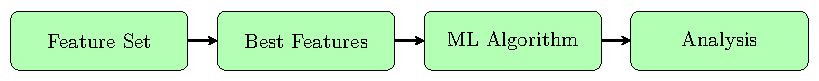
\includegraphics[width=2.5in]{filter-flow.pdf}
		\caption{Filter flow for feature selection}\label{fig:feat-filter-flow}
	\end{center}
\end{figure}

\subsection{Hybrid Feature Selection}

While combinatorial feature selection methods sat clearly in the polynomial time hierarchy, hybrid feature selection methods cannot be formulated into nice computational problems. Hybrid methods effectively utilise a oracle subroutine to calculate the distance function, and in doing so effectively imply infinite computing power\footnote{Since an oracle turing machine can simulate all problems even undecidable problems.}.

We can however, formulate the problem and draw connections between integer programming\footnote{also suggesting that there is linear programming and quantum solutions the feature selection problem.}. Consider the following formulation. Here $\mu : \{ 0, 1 \}^{n} \to \R$ is the measure of a feature vector, with inputs $X$ a set of features. Let $v[i]$ denote the $i$'th entry of a vector.

\begin{definition}
	Given vectors $v\in \{0,1\}^{n}$, find $\text{min}\{ k \mid \forall v\in \{0,1\}^{n}, k=\sum_{i\in[n]} v[i] \}$ such that the image $\mu(v)$ is greater than an arbitrary accuracy bound.
\end{definition}

\begin{figure}[h]
	\begin{center}
		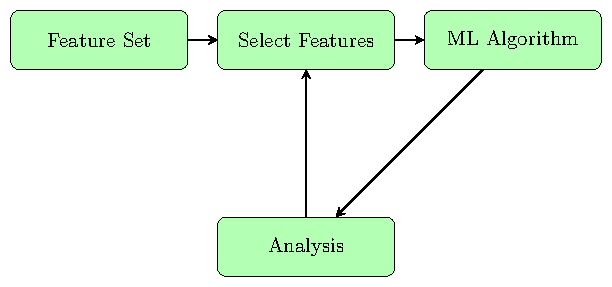
\includegraphics[width=2.5in]{wrapper-flow.pdf}
		\caption{Wrapper flow for feature selection}\label{fig:feat-wrapper-flow}
	\end{center}
\end{figure}

As in~\autoref{fig:feat-wrapper-flow}, wrapper feature selection is distinguishable to filter feature selection because the machine learning algorithm is called as a subroutine.

\subsection{Meta-Heuristics}

Since feature selection is thought to be computationally intractable, meta-heuristics have become an efficient way to compute optimal solutions. Meta-heuristics tend to exist in two broad categories.

\paragraph{Population based meta-heuristics.} A population meta-heuristic is an efficient method at searching a large and high dimensional solution space and finding local optima. This is known to be effective and even provably optimal in high dimensional search spaces due to the `No Free Lunch Theorems'. Population meta-heuristics include, genetic algorithms, ant-colony optimisation algorithms, particle swarm optimisation algorithms.

\paragraph{Local Search based meta-heuristics.} Local search meta-heuristics are algorithms that attempt to optimise an objective function globally. The main drawback is that local search procedures have a tendency to \textit{get stuck} optmising a function that is not the actual global optimum. The most popular local search meta-heuristics include hill climbing, tabu search and simulated annealing.

\paragraph{Memetic algorithms.} A memetic algorithm is an algorithm which presents a hybrid approach between local search and population meta-heuristics. The main idea is as follows, first run a genetic algorithm, at each local optimum run a few rounds of a local search meta-heuristic. Repeat the evolutionary process. Memetic algorithms historically have been incredibly effective at tackling optimisation problems. They also include the additional added benefit that a they will always perform better than their counterpart of just a population meta-heuristic or just a local search meta-heuristic, presenting the open problem of applying memetic algorithms to bias mitigation procedures in feature selection.

\subsection{Computational Considerations}

Genetic algorithms for feature selection while prevalent have a non-trivial computational cost even when ignoring implementation details. It was an interesting question to attempt to understand the complexity of each problem and determine for which parameters different algorithms are effective. For a concrete analysis of the combinatorial problem we can direct readers to\cite{MathiesonEtAl2017,CottaMoscato2003}.

In order to understand the complexity of a hybrid algorithm, let $T$ denote the computational cost of a machine learning algorithm. Observe for a vector of $n$ features with each feature being represented in $\{0,1\}^{n}$. Clearly, we will get the trivial upper bound of $O(T\cdot 2^{n})$, since there is $n$ many entries of two states for a brute force search of all possible features. Assume that a genetic algorithm has a population as a positive integer $p$ and $k$ iterations, since the addition of a local search procedure is asymptotically smaller than $p$ and $k$, note that the iterations of a memetic algorithm have the upper bound of $O(T\cdot pk)$ since we have $k$ many generations of enumerating a population of size $p$. Also note that a brute force solution grows proportionally based on the size of the input $n$ features, where a memetic algorithm has a fixed number of iterations. If we fix the population parameter $p=40$ and the generations $k=50$, note that we obtain an algorithm upper bounded by $O(T\cdot pk)$ iterations.

Here we can compare with various input sizes.

\begin{table}[h!]
	\begin{center}
		\begin{tabular}{| c c c |}
			\hline
			Number of Features & Brute-Force ($2^{n}$) & Memetic Alg ($2000$) \\ [0.5ex]
			\hline
			10                 & 1024                  & 2000                 \\
			15                 & 32768                 & 2000                 \\
			100                & $126765060022\ldots$  & 2000                 \\
			1000               & Uncomputable          & 2000                 \\
			\hline
		\end{tabular}
	\end{center}
	\caption{Comparison between brute force and memetic approach}
	\label{table:memetic-brute-force}
\end{table}

Clearly, by~\autoref{table:memetic-brute-force} we gain no improvment over a brute force solution for $n=10$ without adjustment of parameters, however, if $n=100$ the input quickly becomes too large to handle, suggesting better performance for exponentially bigger inputs.

\section{Proposed Solutions}\label{sec:solutions}

Here we give an overview of our solutions to the feature selection process.

\subsection{Memetic Algorithms for Feature Selection}

Our memetic algorithm implementations were based on both the Handbook of Memetic Algorithms\cite{CottaEtAl2018}, and hybrid gradient descent memetic algorithm approaches\cite{ArabAlfi2015}.


\section{Experiments}

In this section, we aim to evaluate the performance of different classifiers, including Decision Trees (DT), Random Forest (RF), Support Vector Machines (SVM), and the XGBoost Classifier, with and without feature optimization using the memetic algorithm. The primary objective is to determine the impact of feature selection on classifer performance in Instagram fake profile detection. The experimental setup involves implementing, tuning, and testing all classifiers with the reduced feature set on a DeepNote Notebook.

\subsection{Experimental Setup}

\subsubsection{Dataset Description}

We utilised two key datasets for training and testing the classifiers: the Kaggle Insta Final dataset and our custom-curated Insta Fake dataset, which includes fake profiles, and the Insta Auto dataset, consisting of automated bot accounts. These datasets offer a diverse range of instances and class distributions, providing a robust foundation for experimentation.

\begin{figure}[h]
	\begin{center}
		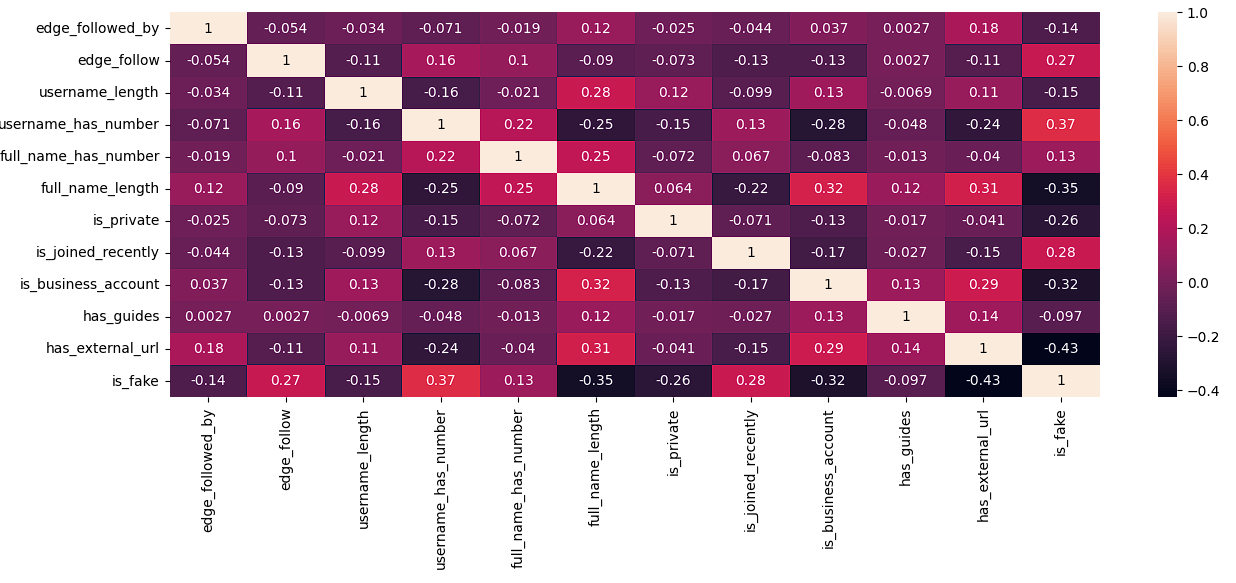
\includegraphics[width=2.5in]{correlation-heatmap}
		\caption{Correlation Heatmap}\label{fig:correlation-heatmap}
	\end{center}
\end{figure}

The correlation heatmap~\autoref{fig:correlation-heatmap} showing the pairwise correlation between different features in the dataset. This visualisation helps identify patterns and relationships between variables, guiding feature selection and preprocessing decisions.

\begin{figure}[h]
	\begin{center}
		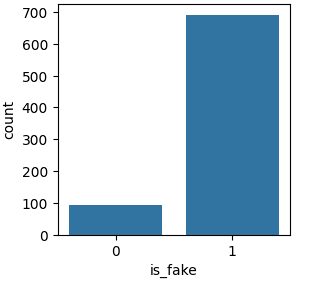
\includegraphics[width=2.5in]{class-distribution}
		\caption{Class Distribution Bar Chart}\label{fig:class-distribution}
	\end{center}
\end{figure}

The bar chart~\autoref{fig:class-distribution} displays the class distribution within the dataset based on the `is fake' label. This visualisation illustrates the balance or imbalance between fake and genuine profiles, providing insights into potential class distribution issues for classification tasks.

\subsection{Preprocessing}

Preprocessing steps included data cleaning, normalisation, and feature engineering to ensure the datasets were suitable for training the classifiers. Additionally, hyper-parameter tuning was performed for penalty factors directly correlating to feature optimisation and the number of features selected for each cycle.

\subsection{Implementation Details}

Before implementing the memetic algorithm for feature optimisation with each classifier, We first tuned the memetic algorithm using the Decision Tree classifier. The parameters and configurations of the memetic algorithm were customised to optimise feature selection specifically for the Decision Tree classifier. There were three implementations of the memetic algorithm, each incorporating different features and achieving different results.

We implemented three different mememtic algorithms, one memetic algorithm focused on generating the smallest feature set by tuning the objective function to place higher weight on smaller feature sets. Another memetic algorithm focused on generating the highest accuracy score. Finally, our last memetic algorithm focused on performance by exploiting parallelism and the efficient ocaml language. The implementations can be found in the appendix.

Once tuned, the parameters of the genetic algorithm were then utilised for feature optimisation with the other classifiers, including Random Forest, SVM, and XGBoost. This approach ensured that the genetic algorithm tailored to each classifier's requirements, maximising its effectiveness in selecting relevant features.

\subsection{Optimal Feature Selection}

Using the insta final dataset, we started with the following 12 features.

\begin{enumerate}
\item Edge Followed By
\item Edge Follow
\item Username Length
\item Username Has Numbers
\item Full Name Length
\item Full Name Has Numbers
\item Is Private
\item Is Recently Joined
\item Has Channel
\item Is Business Account
\item Has Guides
\item Has External Url
\end{enumerate}

We managed an impressive $50\%$ reduction of features by reducing the dataset to 6 features, listed below.

\begin{enumerate}
\item Edge Followed By
\item Edge Follow
\item Username Has Numbers
\item Is Private
\item Is Recently Joined
\item Is Business Account
\end{enumerate}

\subsection{Experimental results}

When we compare the results of different classifiers we see we obtain a marginal loss of performance and accuracy of the classifiers, remembering that while these results are indicative of the scores on the dataset, they are not indicative of the generality of the model. In this sense any score above 90 percent accuracy is a good result, but the key improvement is the reduced feature set.

\subsubsection{XG-Boost}

For the xg-boost classifier, in general we found a negligible performance loss with the reduced feature set.

\begin{table}[h!]
    \begin{center}
	\begin{tabular}{| c | c c |}
		\hline
		Features & F1-Score & AUC-Score\\ [0.5ex]
		\hline
		All Features & 0.97 & 0.99    \\
		Reduced Features & 0.95 & 0.99     \\[1ex]
		\hline
	\end{tabular}
\end{center}
	\caption{Results of the XGBoost Classifier}
	\label{table:xgboost-results}
\end{table}

We can see that there is marginal difference in~\autoref{table:xgboost-results}. Additionally, we can see by the ROC curves, that the loss is marginal compared to the significant gain of a 50 percent feature reduction from~\autoref{fig:xg-roc-curve} to~\autoref{fig:xg-roc-curve-reduced}.

\begin{figure}[h]
	\begin{center}
		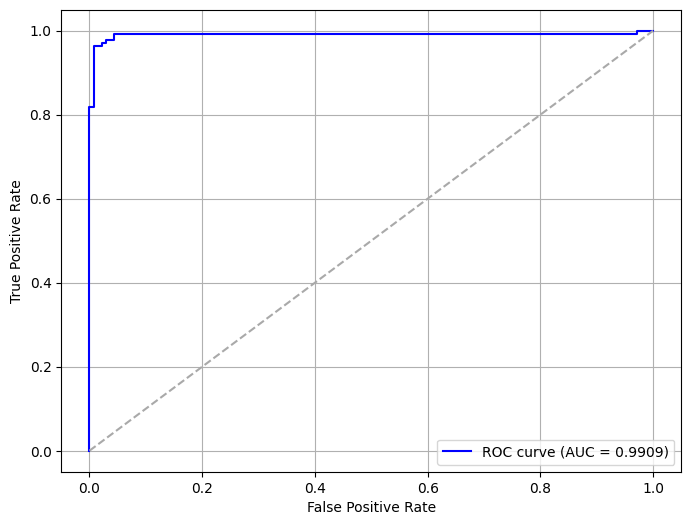
\includegraphics[width=2.5in]{xg-roc-curve}
		\caption{XGBoost ROC Curve with all features}\label{fig:xg-roc-curve}
	\end{center}
\end{figure}

\begin{figure}[h]
	\begin{center}
		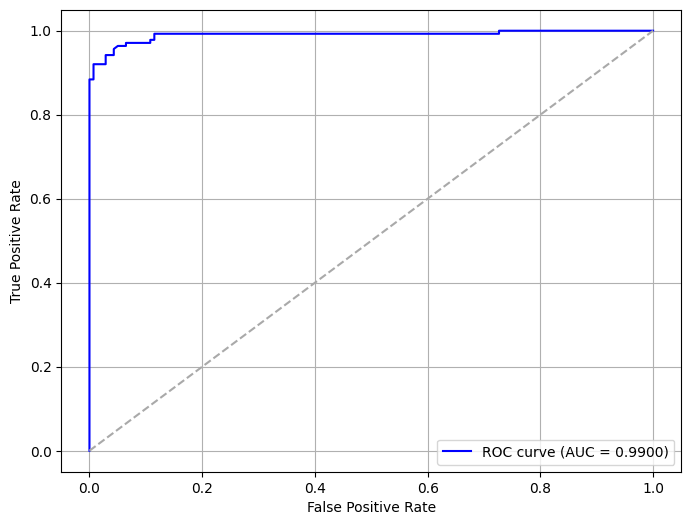
\includegraphics[width=2.5in]{xg-roc-curve-reduced}
		\caption{XGBoost ROC Curve with reduced features}\label{fig:xg-roc-curve-reduced}
	\end{center}
\end{figure}

\subsubsection{SVM}

Support vector machine classifiers in general and unsurprisingly perform worse than XGBoost, but they do also have a marginal decrease in accuracy for a reduced feature set.

\begin{table}[h!]
    \begin{center}
	\begin{tabular}{| c | c c |}
		\hline
		Features & F1-Score & AUC-Score\\ [0.5ex]
		\hline
		All Features & 0.94 & 0.98    \\
		Reduced Features & 0.91 & 0.98     \\[1ex]
		\hline
	\end{tabular}
\end{center}
	\caption{Results of the SVM Classifier}
	\label{table:svm-results}
\end{table}

Again, we only see a 0.03 decrese in the F1-score within~\autoref{table:svm-results}. This is a small and negligible tradeoff, and when we compare the ROC curves~\autoref{fig:svm-roc-curve} and~\autoref{fig:svm-roc-curve-reduced}, we see the difference is even slimmer.

\begin{figure}[h]
	\begin{center}
		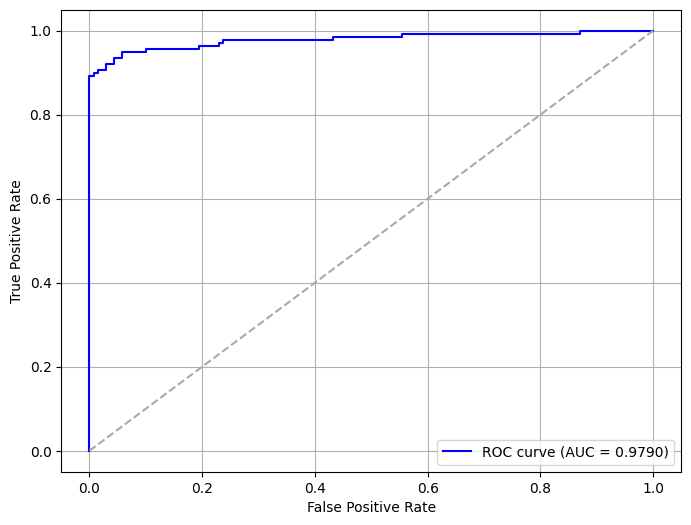
\includegraphics[width=2.5in]{svm-roc-curve}
		\caption{SVM ROC Curve with all features}\label{fig:svm-roc-curve}
	\end{center}
\end{figure}

\begin{figure}[h]
	\begin{center}
		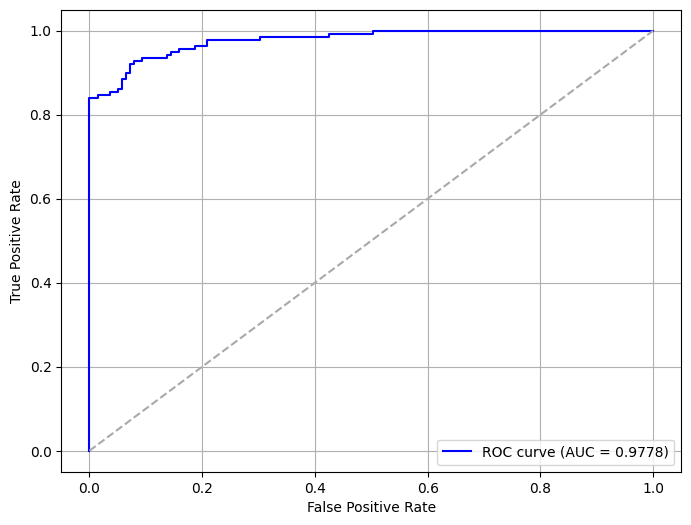
\includegraphics[width=2.5in]{svm-roc-curve-reduced}
		\caption{SVM ROC Curve with reduced features}\label{fig:svm-roc-curve-reduced}
	\end{center}
\end{figure}



\section{Conclusion}

% An example of a floating figure using the graphicx package.
% Note that \label must occur AFTER (or within) \caption.
% For figures, \caption should occur after the \includegraphics.
% Note that IEEEtran v1.7 and later has special internal code that
% is designed to preserve the operation of \label within \caption
% even when the captionsoff option is in effect. However, because
% of issues like this, it may be the safest practice to put all your
% \label just after \caption rather than within \caption{}.
%
% Reminder: the "draftcls" or "draftclsnofoot", not "draft", class
% option should be used if it is desired that the figures are to be
% displayed while in draft mode.
%
%\begin{figure}[!t]
%\centering
%\includegraphics[width=2.5in]{myfigure}
% where an .eps filename suffix will be assumed under latex,
% and a .pdf suffix will be assumed for pdflatex; or what has been declared
% via \DeclareGraphicsExtensions.
%\caption{Simulation results for the network.}
%\label{fig_sim}
%\end{figure}

% Note that the IEEE typically puts floats only at the top, even when this
% results in a large percentage of a column being occupied by floats.


% An example of a double column floating figure using two subfigures.
% (The subfig.sty package must be loaded for this to work.)
% The subfigure \label commands are set within each subfloat command,
% and the \label for the overall figure must come after \caption.
% \hfil is used as a separator to get equal spacing.
% Watch out that the combined width of all the subfigures on a
% line do not exceed the text width or a line break will occur.
%
%\begin{figure*}[!t]
%\centering
%\subfloat[Case I]{\includegraphics[width=2.5in]{box}%
%\label{fig_first_case}}
%\hfil
%\subfloat[Case II]{\includegraphics[width=2.5in]{box}%
%\label{fig_second_case}}
%\caption{Simulation results for the network.}
%\label{fig_sim}
%\end{figure*}
%
% Note that often IEEE papers with subfigures do not employ subfigure
% captions (using the optional argument to \subfloat[]), but instead will
% reference/describe all of them (a), (b), etc., within the main caption.
% Be aware that for subfig.sty to generate the (a), (b), etc., subfigure
% labels, the optional argument to \subfloat must be present. If a
% subcaption is not desired, just leave its contents blank,
% e.g., \subfloat[].


% An example of a floating table. Note that, for IEEE style tables, the
% \caption command should come BEFORE the table and, given that table
% captions serve much like titles, are usually capitalized except for words
% such as a, an, and, as, at, but, by, for, in, nor, of, on, or, the, to
% and up, which are usually not capitalized unless they are the first or
% last word of the caption. Table text will default to \footnotesize as
% the IEEE normally uses this smaller font for tables.
% The \label must come after \caption as always.
%
%\begin{table}[!t]
%% increase table row spacing, adjust to taste
%\renewcommand{\arraystretch}{1.3}
% if using array.sty, it might be a good idea to tweak the value of
% \extrarowheight as needed to properly center the text within the cells
%\caption{An Example of a Table}
%\label{table_example}
%\centering
%% Some packages, such as MDW tools, offer better commands for making tables
%% than the plain LaTeX2e tabular which is used here.
%\begin{tabular}{|c||c|}
%\hline
%One & Two\\
%\hline
%Three & Four\\
%\hline
%\end{tabular}
%\end{table}


% Note that the IEEE does not put floats in the very first column
% - or typically anywhere on the first page for that matter. Also,
% in-text middle ("here") positioning is typically not used, but it
% is allowed and encouraged for Computer Society conferences (but
% not Computer Society journals). Most IEEE journals/conferences use
% top floats exclusively.
% Note that, LaTeX2e, unlike IEEE journals/conferences, places
% footnotes above bottom floats. This can be corrected via the
% \fnbelowfloat command of the stfloats package.


\appendix

\section{Code}

Here is the implementations.

\begin{itemize}
	\item DeepNote Code, managed by Raeyen, Group Contribution \href{https://deepnote.com/workspace/yes-c049-5ed54f34-9a07-49d4-91a2-b1419cbace6e/project/Raeyen-Nuttalls-Untitled-project-15377316-ffd4-45cc-9912-cba9081d5b2e/notebook/Memetic%20Algorithm-412d34e5cc8042b893fdd10bccc6b6c3}{Deep Note Notebook}
	\item Repository for alternative code and OCaml Multi-Threaded memetic algorithm \href{https://github.com/UTS-Projects-2021-2025/insta-fake-profile-detection}{Insta Fake Profile Detection Repository}.
\end{itemize}

% use section* for acknowledgment
\section*{Acknowledgment}


The authors would like to thank...





% trigger a \newpage just before the given reference
% number - used to balance the columns on the last page
% adjust value as needed - may need to be readjusted if
% the document is modified later
%\IEEEtriggeratref{8}
% The "triggered" command can be changed if desired:
%\IEEEtriggercmd{\enlargethispage{-5in}}

\newpage
\printbibliography



% that's all folks
\end{document}


